\documentclass[a4paper,12pt]{report}
\usepackage{styles/fbe_tez}
\usepackage[utf8x]{inputenc} % To use Unicode (e.g. Turkish) characters
\renewcommand{\labelenumi}{(\roman{enumi})}
\usepackage{amsmath, amsthm, amssymb}
 % Some extra symbols
\usepackage[bottom]{footmisc}
\usepackage{cite}
\usepackage{url}
\usepackage{graphicx}
\usepackage{longtable}
\graphicspath{{figures/}} % Graphics will be here

\usepackage{multirow}
\usepackage{subfigure}
\usepackage{algorithm}
\usepackage{algorithmic}

\usepackage{booktabs}
\usepackage{tabularx}
\usepackage{tikz}
\usetikzlibrary{positioning,arrows.meta,shapes.geometric}
\newcommand{\code}[1]{\texttt{#1}}

\begin{document}

% Title Page
\title{CMPE 491 \\ Serving-Aware Cost Modeling for Semantic Operators}
\author{
Yusuf Kaan Akçay \\ \\
Advisor: \\
Prof. Atay Özgövde
}
\date{}
\maketitle{}
\pagenumbering{roman}
\tableofcontents

%======================================================================
\chapter{INTRODUCTION}
\pagenumbering{arabic}

LLM-powered query processing systems expose \emph{semantic operators}: map, filter, join or
extract steps whose logic is a natural-language instruction executed by a large language model
(LLM). Palimpzest \cite{palimpzest} and LOTUS \cite{lotus} are two such systems. Because a query can
be executed in many ways (different models per operator, ensembles such as Mixture-of-Agents,
different prompt strategies), these systems include a cost-based optimizer. Abacus
\cite{russo2025abacus}, the optimizer of Palimpzest, estimates the quality, cost and latency of
candidate operators by sampling them on a validation set and chooses a plan for a user policy such as
``maximize quality'' or ``minimize cost''.

The cost model is additive: an operator costs its input and output tokens times the model's API
price, and a plan costs the sum of its operators. This is accurate for a pay-per-token API. It is not
obviously accurate when an organization serves open models on its own GPUs, for example for privacy
reasons or at high volume. There, the cost is GPU time, and GPU time for the same tokens depends on
(i)~how many requests the server can batch together, (ii)~how many prompt tokens are served from the
prefix cache, and (iii)~whether the model a step needs is already in GPU memory. Liu et
al.~\cite{liu2025optimizing} showed that reordering the rows and columns of an LLM query increases
prefix-cache reuse and speeds it up by up to 3.4$\times$ without changing the token count, an effect a
token-based estimate cannot see.

This project measures how far the two cost views diverge. We built a portable harness that serves
two open models (Llama-3.1-8B-Instruct and Qwen2.5-7B-Instruct) on a single NVIDIA L4 GPU, switching
between them with vLLM's sleep mode, and ran two experiments on the CUAD contract-review benchmark:
four manually specified plans under two execution strategies, and the plans that Abacus itself
chooses. So far, execution order alone changes GPU time by 7.8--11.5$\times$ at identical token cost,
the plan that is cheapest at API prices is not the cheapest on the GPU, and the plan Abacus chooses
for maximum quality costs 9.9$\times$ more at GPU prices than at API prices.

\section{Broad Impact}

Organizations that run LLM-based data processing choose between paying an API per token and serving
open models on their own hardware. Semantic query optimizers are built for the first case. If their
plans are far from optimal in the second case, a self-hosting organization pays for it in GPU time,
energy and latency without the optimizer noticing. Quantifying this gap tells system builders whether
optimizers need a serving-aware cost model, and tells practitioners which plan choices (one model
versus several, operator-by-operator execution) matter most when they self-host.

The measurement harness is open source and runs the same Docker image on a laptop, a cloud VM, a
Slurm cluster (TRUBA) or Kubernetes, so the experiments can be repeated on other GPUs and models.

\section{Ethical Considerations}

\begin{itemize}
\item \textbf{Data.} CUAD \cite{hendrycks2021cuad} consists of commercial contracts that were filed
publicly; it contains no data collected from individuals for this project, and no user data is
processed.
\item \textbf{Models.} Only openly released model weights are used: Llama-3.1-8B-Instruct under the
Llama 3.1 Community License (access granted through Hugging Face) and Qwen2.5-7B-Instruct under
Apache 2.0.
\item \textbf{Resources.} GPU time costs money and energy. Every cloud run is limited by a maximum run
duration, VMs delete themselves after a run, and a billing guard disables the project's billing once
the free credits are used up.
\item \textbf{Secrets.} The Hugging Face access token is kept in a secret manager and never stored in
code or configuration files.
\item \textbf{Use of AI tools.} The literature search and screening, parts of the implementation and
the writing of this report were carried out with the help of an AI assistant (Claude); all results
reported here come from our own measurements.
\end{itemize}

%======================================================================
\chapter{PROJECT DEFINITION AND PLANNING}

\section{Project Definition}

\textbf{Research question.} Does a semantic query plan that is optimal under API pricing remain
optimal when executed on a self-hosted vLLM server, and if not, how far do the two cost views
diverge?

The project tests three hypotheses (Table~\ref{table:hypotheses}). The deliverables are the
measurement harness, the integration of Abacus with self-hosted models, the measurements on CUAD,
and an analysis comparing the plans ranked by API cost with the plans ranked by GPU cost.

\begin{table}[thbp]
\vskip\baselineskip
\caption{Hypotheses.}
\begin{center}
\small
\begin{tabularx}{\linewidth}{@{}lXX@{}}
\toprule
& Hypothesis & Test \\
\midrule
H1 & The self-hosted cost of multi-model plans (mixed, Mixture-of-Agents) depends on execution order; switching models per record can push them off the Pareto frontier. & Run the same plan record by record and operator by operator; compare GPU time and model switches. \\
H2 & Running operators that share a model back to back increases prefix-cache reuse, which an additive cost model ignores. & Measure prefix-cache hits and GPU time with the token count fixed. \\
H3 & Plans ranked by API cost and by GPU cost are ordered differently. & Kendall's $\tau$ between the two rankings; compare the two Pareto frontiers. \\
\bottomrule
\end{tabularx}
\label{table:hypotheses}
\end{center}
\end{table}

\section{Project Planning}

\subsection{Project Time and Resource Estimation}

Table~\ref{table:timeline} lists the work packages and their status.

\begin{table}[thbp]
\vskip\baselineskip
\caption{Work packages.}
\begin{center}
\small
\begin{tabularx}{\linewidth}{@{}Xll@{}}
\toprule
Work package & Period & Status \\
\midrule
Literature review & October 2026 & Done \\
vLLM measurement tooling (laptop GPU) & October 2026 & Done \\
Portable harness, GCP pipeline, billing guard & November 2026 & Done \\
First measurements on the L4 (0.5B and 8B models) & November 2026 & Done \\
CUAD workload, prompts and F1 & November 2026 & Done \\
CUAD control experiment (pilot and full run) & November 2026 & Done \\
Abacus integration with self-hosted models & November 2026 & Done \\
Abacus runs (pilot, then all three policies) & November--December 2026 & In progress \\
Repeats, KV-cache experiments, single-server baseline & December 2026 & Planned \\
Second workload, final analysis, final report & CMPE 492 & Planned \\
\bottomrule
\end{tabularx}
\label{table:timeline}
\end{center}
\end{table}

\textbf{Compute.} All GPU experiments run on Google Cloud on a \code{g2-standard-16} VM (one NVIDIA L4
with 24\,GB, 16 vCPUs, 64\,GB RAM), whose on-demand price is 1.147\,USD per hour
\cite{gcppricing}. The runs so far took roughly 17 VM-hours (CUAD full run 7.7\,h, CUAD pilot 2.0\,h,
first Abacus run about 6\,h, smaller tests about 1\,h), about 20--25\,USD at that price. This is
an estimate from run durations, not a billing figure. The work is covered by Google Cloud's free-trial
credit of 300\,USD.

\textbf{Software.} vLLM 0.30.0, Palimpzest 1.5.3, Python, Docker, Google Cloud (Compute Engine,
Cloud Build, Artifact Registry, Cloud Storage, Secret Manager). Model weights are downloaded from
Hugging Face.

\subsection{Success Criteria}

\begin{enumerate}
\item Each of H1--H3 is supported or rejected by measurements on CUAD, with the run data and
configuration published so that the result can be reproduced.
\item The plans Abacus chooses for its three policies (MaxQuality, MinCost, MinTime) are executed on
the self-hosted models, and their GPU cost is compared with their API cost and with the control
experiment.
\item Quality is measured with the same F1 as Abacus, so that our numbers are comparable with its
paper.
\item The harness runs unchanged on at least two environments (a laptop GPU and a cloud GPU).
\end{enumerate}

\subsection{Risk Analysis}

\begin{table}[thbp]
\vskip\baselineskip
\caption{Risks.}
\begin{center}
\small
\begin{tabularx}{\linewidth}{@{}XX@{}}
\toprule
Risk & Mitigation \\
\midrule
L4 GPUs are out of stock in a zone (observed often). & VM creation retries six zones in two regions every 10 minutes for up to 3 hours. \\
Cloud cost exceeds the free credit. & Billing guard disables billing automatically; every VM has a maximum run duration and deletes itself. \\
Two models do not fit on one 24\,GB GPU. & Sleep mode keeps one model's weights in CPU memory; the GPU memory share was tuned (0.85). \\
A run is interrupted (preemption, time limit). & Deterministic run IDs: a restarted run skips finished runs; results are uploaded every 10 minutes. \\
Abacus integration breaks on self-hosted models (it assumes one vLLM model and API prices). & Runtime patches, each tested against a stub vLLM server before GPU runs. \\
Abacus runs take longer than planned (observed: 6\,h were not enough). & Pilot runs on a subset first; output-token limit and fewer concurrent requests. \\
\bottomrule
\end{tabularx}
\label{table:risks}
\end{center}
\end{table}

\subsection{Team Work (if applicable)}

This is an individual project.

%======================================================================
\chapter{RELATED WORK}

We followed the citation trees of the two papers this project builds on \cite{liu2025optimizing,
russo2025abacus} three levels deep on Semantic Scholar (56 direct citations, about 2,170 papers in
total), filtered them by keyword, and read the closest $\sim$20 papers.

Two lines of work exist side by side (Table~\ref{table:related}). Systems that \emph{choose} a plan
do not model the serving state of the GPU (which model is loaded, what is cached); systems that
\emph{execute} LLM workloads efficiently on GPUs take the plan as given. We found no work that
measures this gap for semantic operator optimizers. The contribution of this project is therefore a
measurement, not a new system.

\begin{table}[thbp]
\vskip\baselineskip
\caption{Closest related work.}
\begin{center}
\small
\begin{tabularx}{\linewidth}{@{}llX@{}}
\toprule
Work & Side & Relation to this project \\
\midrule
Halo \cite{halo} & Execution & Cost model covers prefill/decode, cache sharing and model loading, but takes the model assignment as given. \\
Kalypso \cite{kalypso} & Execution & Shares KV cache across semantic operators; single model, no plan choice. \\
Helium \cite{helium} & Execution & Cache- and batch-aware scheduling; single model. \\
MOSAIC \cite{mosaic} & Execution & Schedules Mixture-of-Agents on limited GPUs; no plan choice. \\
Stretto \cite{stretto} & Plan choice & Models operator cost by measured time; no model switching, no API vs.\ GPU comparison. \\
BlendSQL v0.1.0 \cite{blendsql} & Plan choice & Compares open models on a local GPU with APIs; rule-based optimizer. \\
NeurEngine \cite{aixdb} & Vision & Names model placement outside the optimizer as an open problem. \\
Akillioglu \cite{akillioglu2025} & Vision & Proposes a cost model that includes KV-cache hits; SQL, single model. \\
Yildiz et al. \cite{multimodelsched} & Switching & Report 4--5\,s to reload an 8B model. \\
\bottomrule
\end{tabularx}
\label{table:related}
\end{center}
\end{table}

%======================================================================
\chapter{METHODOLOGY}

\section{Two Experiments}

\textbf{Control experiment (fixed plans).} We specify four plans and two execution strategies
ourselves (Table~\ref{table:plans}). Because we choose the plans, we can isolate the effect of
batching, prefix caching and model switching. Its results also serve as the reference for
interpreting the plans Abacus chooses.

\textbf{Main experiment (Abacus).} We give Abacus the API list prices of the two models and let it
choose a plan for each policy (MaxQuality, MinCost, MinTime). We then execute the chosen plan on the
self-hosted server and measure its GPU time.

In both, every plan is priced twice: tokens $\times$ API list price, and measured GPU time $\times$
hourly GPU price. The two rankings are compared with Kendall's $\tau$ and two Pareto frontiers
(quality against each cost).

\section{Models and Prices}

The models are Llama-3.1-8B-Instruct and Qwen2.5-7B-Instruct. API prices are Together AI list
prices: 0.18\,USD per million tokens for Llama-3.1-8B and 0.30\,USD for Qwen2.5-7B-Instruct-Turbo,
for both input and output \cite{togetherllama, togetherqwen}. The GPU price is the on-demand price
of the \code{g2-standard-16} VM, 1.147\,USD per hour \cite{gcppricing}; this is the price of the whole
VM, not only the GPU.

\begin{table}[thbp]
\vskip\baselineskip
\caption{Plans and execution strategies of the control experiment.}
\begin{center}
\small
\begin{tabularx}{\linewidth}{@{}lX@{}}
\toprule
Plan & Definition \\
\midrule
\code{all\_llama} & Both operators run on Llama. \\
\code{all\_qwen} & Both operators run on Qwen. \\
\code{mixed} & One model per operator (operator A on Qwen, operator B on Llama). \\
\code{moa} & Operator A on Qwen; operator B as Mixture-of-Agents: Llama and Qwen propose, Llama aggregates. \\
\midrule
Strategy & Definition \\
\midrule
\code{naive} & Record by record; switches the model whenever the next step needs the other one. \\
\code{batched} & Operator by operator; each model is woken once and processes all records. \\
\bottomrule
\end{tabularx}
\label{table:plans}
\end{center}
\end{table}

Single-model plans never switch models, so their naive/batched gap isolates batching and caching;
for multi-model plans the switch cost comes on top.

\section{Workload: CUAD}

CUAD \cite{hendrycks2021cuad} is a legal contract-review dataset with 41 clause categories (for
example parties, governing law, non-compete) annotated as text spans. We select 25 test contracts
exactly as Abacus's CUAD demo does (titles shuffled with seed 0) and split them into chunks of at
most 4,000 characters, giving 160 chunks; 99\% of the labeled spans fall inside a single chunk. For
Abacus's sampling we prepare 25 training contracts the same way (313 chunks). In the control
experiment the 41 categories are extracted by two operators (21 and 20 categories); in the Abacus
experiment by Abacus's own single operator over all 41.

Quality is precision, recall and F1 with Abacus's span matching: a prediction matches a label when
their Jaccard similarity is at least 0.15 (for Parties a substring also counts), and predictions are
merged per contract.

\section{What Is Held Fixed and What Is Measured}

Held fixed: the configuration (its hash is stored with every run), GPU type, vLLM version (0.30.0),
image digest, temperature 0 in the control experiment, and an empty prefix cache with the first
model awake at the start of every run. Measured: wall-clock GPU time, number and duration of model
switches, prompt, completion and cached tokens per model, prefix-cache queries and hits from vLLM's
\code{/metrics} endpoint, and F1.

%======================================================================
\chapter{REQUIREMENTS SPECIFICATION}

The system is an experiment harness used by one researcher; its use cases are shown in
Figure~\ref{fig:usecase}.

\begin{figure}[h!]
\centering
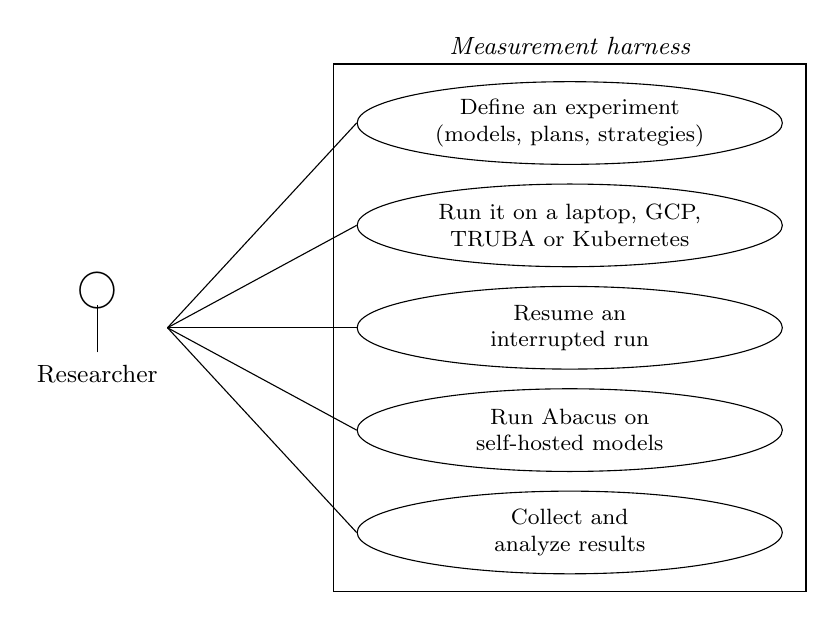
\begin{tikzpicture}[
  uc/.style={ellipse, draw, minimum width=5.4cm, minimum height=1.05cm, inner sep=1pt, font=\footnotesize, align=center},
  actor/.style={font=\small, align=center}]
\node[actor] (r) at (0,0) {\Large$\bigcirc$\\[-2pt]\rule{0.4pt}{0.6cm}\\Researcher};
\node[uc] (u1) at (6, 2.6) {Define an experiment\\(models, plans, strategies)};
\node[uc] (u2) at (6, 1.3) {Run it on a laptop, GCP,\\TRUBA or Kubernetes};
\node[uc] (u3) at (6, 0.0) {Resume an\\interrupted run};
\node[uc] (u4) at (6,-1.3) {Run Abacus on\\self-hosted models};
\node[uc] (u5) at (6,-2.6) {Collect and\\analyze results};
\draw (3.0,-3.35) rectangle (9.0,3.35);
\node[font=\small\itshape, anchor=south] at (6,3.35) {Measurement harness};
\foreach \u in {u1,u2,u3,u4,u5} \draw (r.east) -- (\u.west);
\end{tikzpicture}
\caption{Use cases of the measurement harness.}
\label{fig:usecase}
\end{figure}

\textbf{Functional requirements.}
\begin{enumerate}
\item Start one vLLM server per model and keep exactly one awake on a shared GPU.
\item Execute every (plan, strategy, repeat) combination of a configuration from the same starting
state, and record time, model switches, tokens, prefix-cache counters and F1 for each.
\item Skip finished runs when restarted.
\item Run Palimpzest/Abacus against the self-hosted models and record the plan it chooses, its API
cost and the measured GPU cost.
\end{enumerate}

\textbf{Non-functional requirements.}
\begin{enumerate}
\item Reproducibility: the same image and configuration give the same setup on every environment;
the configuration hash, vLLM version and image digest are stored with every result.
\item Cost control: cloud runs are bounded in time and spending.
\item No secrets in the code or configuration.
\end{enumerate}

%======================================================================
\chapter{DESIGN}

\section{Information Structure}

The harness has no database. Each run appends one JSON record to \code{runs.jsonl} (control
experiment) or \code{pz\_runs.jsonl} (Abacus); Table~\ref{table:record} lists the fields of a
control-experiment record.

\begin{table}[thbp]
\vskip\baselineskip
\caption{Fields of one run record (\code{runs.jsonl}).}
\begin{center}
\small
\begin{tabularx}{\linewidth}{@{}lX@{}}
\toprule
Field & Meaning \\
\midrule
\code{run\_id}, \code{plan}, \code{strategy}, \code{repeat} & Which run; \code{run\_id} is a hash of experiment, plan, strategy, repeat and configuration \\
\code{env}, \code{gpu\_name}, \code{vllm\_version}, \code{image\_digest}, \code{config\_hash} & Where and with what it ran \\
\code{wall\_time\_s} & GPU time of the run \\
\code{n\_model\_switches}, \code{switch\_time\_s} & Sleep/wake count and time \\
\code{usage} & Prompt, completion and cached tokens per model \\
\code{prefix\_cache} & Prefix-cache queries and hits per server \\
\code{quality} & Precision, recall, F1 and the number of unparsable answers \\
\bottomrule
\end{tabularx}
\label{table:record}
\end{center}
\end{table}

\section{Information Flow}

Figure~\ref{fig:flow} shows how a cloud run flows from the researcher's command to the results.

\begin{figure}[h!]
\centering
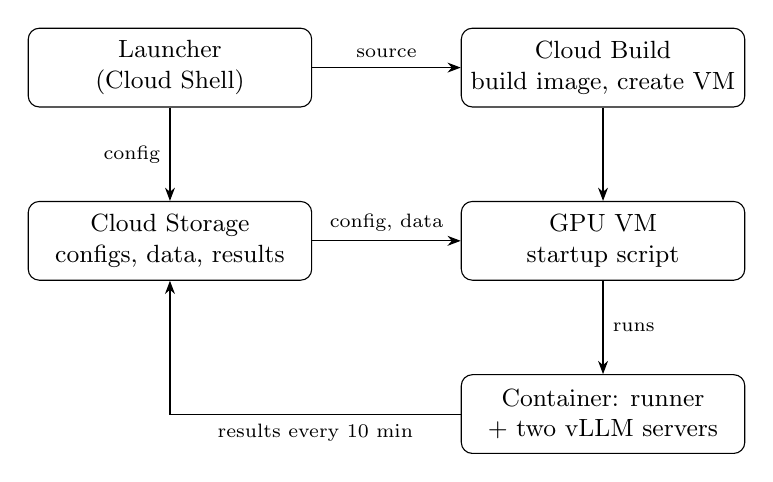
\begin{tikzpicture}[
  box/.style={draw, rounded corners, align=center, font=\small, minimum width=3.6cm, minimum height=1cm},
  lab/.style={font=\scriptsize},
  >={Stealth}]
\node[box] (l) at (0,0) {Launcher\\(Cloud Shell)};
\node[box] (cb) at (5.5,0) {Cloud Build\\build image, create VM};
\node[box] (gcs) at (0,-2.2) {Cloud Storage\\configs, data, results};
\node[box] (vm) at (5.5,-2.2) {GPU VM\\startup script};
\node[box] (c) at (5.5,-4.4) {Container: runner\\+ two vLLM servers};
\draw[->] (l) -- node[lab, above]{source} (cb);
\draw[->] (l) -- node[lab, left]{config} (gcs);
\draw[->] (cb) -- (vm);
\draw[->] (gcs) -- node[lab, above]{config, data} (vm);
\draw[->] (vm) -- node[lab, right]{runs} (c);
\draw[->] (c.west) -| node[lab, below, pos=0.25]{results every 10 min} (gcs.south);
\end{tikzpicture}
\caption{Information flow of a cloud run. The VM deletes itself after uploading the final results.}
\label{fig:flow}
\end{figure}

Inside the container, a run of the control experiment wakes the model each step needs, sends its
requests, and records the counters. In the Abacus experiment, Palimpzest sends requests for both
models to a proxy, which wakes the requested model and forwards the request to its server.

\section{System Design}

Table~\ref{table:modules} lists the modules of the harness.

\begin{table}[thbp]
\vskip\baselineskip
\caption{Modules of the harness.}
\begin{center}
\small
\begin{tabularx}{\linewidth}{@{}lX@{}}
\toprule
Module & Responsibility \\
\midrule
\code{config.py} & Loads the YAML configuration, builds the run matrix and run IDs \\
\code{servers.py} & Starts the vLLM servers, sleep/wake, times model switches \\
\code{metrics.py} & Reads prefix-cache counters from \code{/metrics} \\
\code{plans.py} & Executes a plan under the naive or batched strategy \\
\code{workloads.py}, \code{cuad.py} & Loads the workload; CUAD categories, answer parsing and F1 \\
\code{runner.py} & Entry point: resume, run, write results \\
\code{proxy.py} & One OpenAI-compatible endpoint for both models; wakes the requested model \\
\code{pz\_runner.py}, \code{pz\_query.py} & Abacus experiment: runs Palimpzest against the proxy and records the results \\
\code{launch/} & Launchers for Docker, GCP, TRUBA (Slurm) and Kubernetes \\
\bottomrule
\end{tabularx}
\label{table:modules}
\end{center}
\end{table}

\section{User Interface Design (if applicable)}

Not applicable: the harness is used from the command line, and experiments are described in YAML
files.

%======================================================================
\chapter{IMPLEMENTATION AND TESTING}

\section{Implementation}

\textbf{Harness.} The runner starts one vLLM server per model and keeps exactly one awake using
vLLM's sleep mode \cite{kwon2023vllm}: a sleeping server moves its weights to CPU memory and drops its
KV cache, so the two models share one 24\,GB L4. Every (plan, strategy, repeat) combination is run
from the same starting state and appended as one JSON line.

\textbf{Abacus integration.} Palimpzest 1.5.3 runs in its own Python environment inside the image.
Running Abacus on self-hosted models needed six changes, all applied at runtime without modifying the
installed package:
\begin{enumerate}
\item Palimpzest allows only one vLLM model per query; this check is lifted.
\item vLLM models are priced at zero; they receive the API list prices from our configuration.
\item Palimpzest records zero input tokens for vLLM models, so cost estimates counted only output
tokens. We count every prompt token at the input price, as an API without a cache discount would.
\item The default validator calls an OpenAI model; ours scores sampled outputs against the CUAD
labels of the training chunks.
\item Palimpzest sets no output-token limit. The proxy adds one to requests without a limit: 2,048
tokens, or fewer when the prompt leaves less room in the context (introduced after the first run;
Section~\ref{sec:abacusres}).
\item Model priors (MMLU-Pro score, speed) are predicted from the Hugging Face model ID rather than
the short served name, which had given both models the same prior.
\end{enumerate}

\section{Testing}

\begin{itemize}
\item \textbf{Stub vLLM server.} A small server that implements the vLLM endpoints the harness uses
and rejects requests sent to a sleeping server. The run matrix, switch counts and resume logic, and
the whole Abacus pipeline, were tested against it before any GPU run.
\item \textbf{Proxy test.} 300 concurrent requests for two models through the proxy: no request may
reach a sleeping server, unknown models are rejected, and the output limit is added and lowered for
long prompts.
\item \textbf{F1.} Our implementation agreed with Abacus's \code{evaluate\_entry} on 3,000 random
cases.
\item \textbf{Measurement checks.} On a laptop GPU (RTX 3050 Ti, 4\,GB) and on the L4, the
per-request cached-token counts and vLLM's server-wide prefix-cache counters agreed in every run.
\item \textbf{Launch scripts.} The VM startup script was tested with stand-ins for the cloud tools
before it was used on a GPU VM.
\end{itemize}

\section{Deployment}

The harness is one Docker image: the official vLLM image plus the harness and a separate Palimpzest
environment. Model weights and access tokens are not part of the image. A cloud run is started from
Cloud Shell with one command, for example:

\begin{verbatim}
PROJECT=<project-id> CONFIG=configs/cuad.yaml MACHINE=g2-standard-16 \
  RETRY=1 ./launch/gcp_gpu_run.sh
\end{verbatim}

The launcher uploads the configuration to Cloud Storage and starts a Cloud Build job that builds the
image and creates the GPU VM (Figure~\ref{fig:flow}). VMs have no external IP; spending is capped by
a budget that disables billing. The same image runs locally with \code{launch/local.sh}, on TRUBA with
\code{launch/truba.sbatch} and on Kubernetes with \code{launch/k8s\_job.yaml}. The code and a README
with these instructions are available at
\url{https://github.com/akcayyusufkaan/serving-aware-semantic-ops}.

%======================================================================
\chapter{RESULTS}

All runs use one NVIDIA L4 on a \code{g2-standard-16} VM and vLLM 0.30.0. Each result is read from
the run's result file (\code{runs.jsonl} or \code{pz\_runs.jsonl}) in the project bucket.

\section{First Measurements on a Small Workload}

A small test workload (six reviews, two operators, 3 repeats differing by less than 1\%) with the two
models showed the effects most clearly (Table~\ref{table:smoke}). One model switch takes 3.03\,s, and
under the naive strategy switches account for 89--91\% of the run time of the multi-model plans.
Switching also discards the prefix cache: \code{mixed} under naive gets no cached prompt tokens,
against 320 under batched.

\begin{table}[thbp]
\vskip\baselineskip
\caption{Small test workload with Llama-3.1-8B and Qwen2.5-7B (mean of 3 repeats).}
\begin{center}
\small
\begin{tabular}{@{}lrrrr@{}}
\toprule
Plan & naive (s) & batched (s) & Ratio & Switch time, naive \\
\midrule
\code{all\_llama} & 4.92 & 0.99 & 5.0$\times$ & -- \\
\code{all\_qwen}  & 4.28 & 0.91 & 4.7$\times$ & -- \\
\code{mixed}      & 37.27 & 3.91 & 9.5$\times$ & 33.3\,s (89\%) \\
\code{moa}        & 39.76 & 6.85 & 5.8$\times$ & 36.4\,s (91\%) \\
\bottomrule
\end{tabular}
\label{table:smoke}
\end{center}
\end{table}

These runs also exposed two constraints of serving two models on one L4. First, vLLM's memory budget
(\code{gpu\_memory\_utilization}) must leave room for the sleeping server, which still holds about
1.8\,GiB of GPU memory (0.80 left no KV cache for Llama, 0.90 did not fit, 0.85 works). Second, the
runs failed on VMs with 32\,GB and 48\,GB of host RAM and succeeded with 64\,GB.

\section{CUAD Control Experiment}

A pilot on the first 40 chunks (6 contracts) confirmed the setup and measured throughput; the full
run on all 160 chunks took 7.7 hours of GPU time for the eight runs (one repeat).
Table~\ref{table:cuad} gives the full run.

\begin{table}[thbp]
\vskip\baselineskip
\caption{CUAD, 25 contracts (160 chunks), one repeat. Cache hit is cached prompt tokens over prompt
tokens. API cost is prompt and completion tokens times the list prices; GPU cost is GPU time times
the hourly VM price.}
\begin{center}
\small
\setlength{\tabcolsep}{4pt}
\begin{tabular}{@{}llrrrrrr@{}}
\toprule
Plan & Strategy & Time (s) & Switches (n/s) & Cache hit & F1 & API (USD) & GPU (USD) \\
\midrule
\code{all\_qwen}  & batched & 352.5   & 0 / 0         & 54\% & 0.665 & 0.155 & 0.112 \\
\code{mixed}      & batched & 447.6   & 1 / 3.1       & 54\% & 0.656 & 0.123 & 0.143 \\
\code{all\_llama} & batched & 557.5   & 0 / 0         & 55\% & 0.645 & 0.093 & 0.178 \\
\code{moa}        & batched & 1,255.8 & 3 / 9.2       & 47\% & 0.550 & 0.248 & 0.400 \\
\midrule
\code{all\_qwen}  & naive   & 4,055.5 & 0 / 0         & 54\% & 0.663 & 0.155 & 1.292 \\
\code{all\_llama} & naive   & 4,374.1 & 0 / 0         & 55\% & 0.653 & 0.093 & 1.394 \\
\code{mixed}      & naive   & 5,129.7 & 319 / 973.6   & 0\%  & 0.654 & 0.123 & 1.635 \\
\code{moa}        & naive   & 11,526.2 & 639 / 1,949.6 & 0\% & 0.555 & 0.248 & 3.673 \\
\bottomrule
\end{tabular}
\label{table:cuad}
\end{center}
\end{table}

\begin{figure}[h!]
\centering
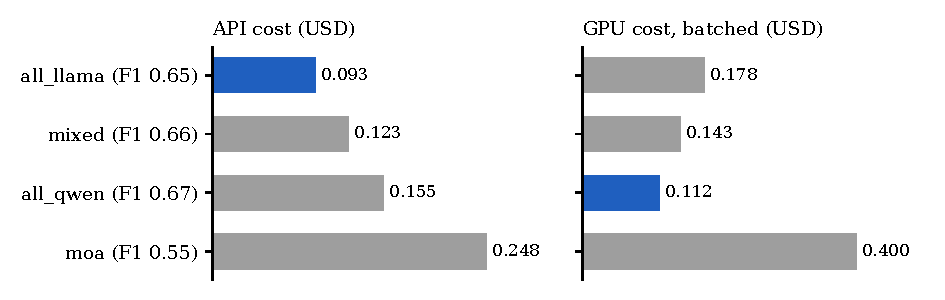
\includegraphics[width=\textwidth]{ranking.pdf}
\caption{The same four plans (batched) ordered by API cost. The cheapest plan in each view is
highlighted: all-Llama at API prices, all-Qwen on the GPU.}
\label{fig:ranking}
\end{figure}

\begin{figure}[h!]
\centering
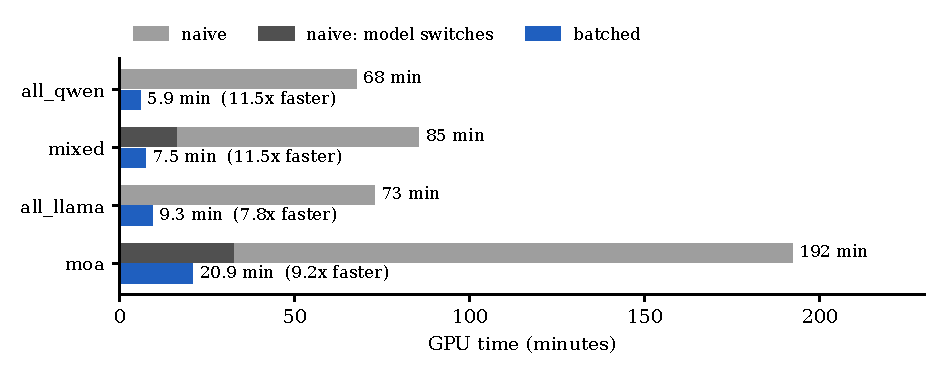
\includegraphics[width=\textwidth]{strategies.pdf}
\caption{GPU time of each plan under the two strategies. Both strategies use the same tokens, so the
API cost of a plan is the same for both.}
\label{fig:strategies}
\end{figure}

\textbf{Finding 1: the cheapest plan at API prices is not the cheapest on the GPU (H3).} At API
prices the order is all-Llama, mixed, all-Qwen, MoA; on the GPU (batched) it is all-Qwen, mixed,
all-Llama, MoA (Figure~\ref{fig:ranking}). All-Llama costs 60\% of all-Qwen at API prices but takes
58\% more GPU time, while both plans use almost the same tokens (443k and 445k prompt tokens). The
difference therefore comes from how fast each model is served, not from the token count. A likely
cause is the KV-cache footprint: 128\,KiB per token for Llama-3.1-8B against 56\,KiB for Qwen2.5-7B.
At the same memory setting vLLM allocated 9,040 tokens of KV cache to Llama and 32,992 to Qwen
(Section~\ref{sec:abacusres}), so Qwen can process more requests at once; the effect on throughput
has not yet been isolated. Kendall's $\tau$ between API cost and GPU time is 0.0 for the batched
plans and 0.33 for the naive ones, with only four plans per ranking.

\textbf{Finding 2: execution order changes GPU time by an order of magnitude at identical API cost
(H1).} Every plan uses the same tokens under both strategies, yet naive takes 7.8--11.5$\times$
longer than batched (Figure~\ref{fig:strategies}). An API cost model assigns both the same cost.

\textbf{Finding 3: at CUAD scale, switching is secondary to batching and caching (H1, H2).} Model
switches take 17--19\% of the naive run time of the multi-model plans, down from 89--91\% on the small
workload, because each record now carries far more work. The larger loss is that naive execution
processes records one at a time, and that every switch empties the prefix cache: naive \code{mixed}
and \code{moa} get no cache hits, against 47--54\% under batched.

\textbf{Finding 4: Pareto frontiers.} With F1 against API cost, all-Llama, mixed and all-Qwen are on
the frontier. With F1 against GPU cost (batched), all-Qwen dominates every other plan, so the
frontier is a single point. MoA, which Abacus selected in all ten of its CUAD trials with API models
\cite{russo2025abacus}, is dominated in both views here: it uses twice the tokens, has the lowest F1
(0.55) and the longest GPU time.

\section{Abacus on the Self-Hosted Models}
\label{sec:abacusres}

The first run on the L4 (all 160 test chunks, sample budget 50, policies MaxQuality, MinCost and
MinTime) completed only the MaxQuality policy before the VM reached its 6-hour limit
(Table~\ref{table:abacus}).

\begin{table}[thbp]
\vskip\baselineskip
\caption{Abacus, MaxQuality policy. Chosen plan: one Mixture-of-Agents operator over all 41
categories, proposers Llama and Qwen, aggregator Qwen. API cost is Palimpzest's own figure at the list
prices; GPU cost is GPU time times the hourly VM price.}
\begin{center}
\footnotesize
\setlength{\tabcolsep}{4pt}
\begin{tabular}{@{}lrrrrr@{}}
\toprule
Phase & Time (s) & Switches (n/s) & API (USD) & GPU (USD) & GPU/API \\
\midrule
Optimization (train chunks) & 4,315.7 & 50 / 151.4 & 0.189 & 1.375 & 7.3$\times$ \\
Execution (160 test chunks) & 7,303.8 & 10 / 32.9  & 0.235 & 2.328 & 9.9$\times$ \\
\bottomrule
\end{tabular}
\label{table:abacus}
\end{center}
\end{table}

\textbf{Abacus again chooses Mixture-of-Agents.} As in all ten of its CUAD trials with API models
\cite{russo2025abacus}, MaxQuality selected a Mixture-of-Agents operator, the plan type that is
dominated in our control experiment.

\textbf{At GPU prices the plan costs an order of magnitude more.} Executing the plan cost 2.33\,USD
at GPU prices against 0.24\,USD at API prices (9.9$\times$); for the fixed Mixture-of-Agents plan in
the control experiment the ratio was 1.6$\times$ (batched).

\textbf{The serving logs show why.} vLLM could allocate only 9,040 tokens of KV cache to Llama
(32,992 to Qwen), so Llama served about one long request at a time, at about 16 output tokens per
second. Palimpzest sets no output limit, and when the run stopped a single running Llama request
occupied about 90\% of that cache. The client timed out on 358 requests after 600\,s, and 34 answers
could not be parsed. These failures likely lower quality as well: F1 was 0.31 (precision 0.59, recall
0.21), so this F1 is not comparable with the control experiment. The proxy now adds an output limit
and Palimpzest sends at most 8 concurrent requests; a pilot on 20 chunks will measure the run time
before the full Abacus run is repeated.

%======================================================================
\chapter{CONCLUSION}

The measurements so far support all three hypotheses on CUAD. The plan that is cheapest at API prices
(all-Llama) is not the cheapest on a self-hosted GPU (all-Qwen), execution order changes GPU time by
7.8--11.5$\times$ at identical API cost, and model switches empty the prefix cache. Abacus, run on the
same self-hosted models, again chose Mixture-of-Agents for maximum quality, a plan that costs an order
of magnitude more at GPU prices than at API prices.

\textbf{Limitations.}
\begin{itemize}
\item The CUAD runs have a single repeat. On the small workload repeats differed by less than 1\%;
additional repeats of the batched runs are planned.
\item Each ranking has four plans, so Kendall's $\tau$ is a weak statistic here; the per-plan
comparison is the main evidence.
\item The GPU price is the price of the whole VM. A different GPU or price would change the absolute
GPU costs but not the ranking by GPU time.
\item Both models share one GPU in every run, including single-model plans, so the sleeping model
reduces the KV cache available to the active one.
\item The cause of the host-RAM failures on smaller VMs has not been identified.
\item The first Abacus run covers one policy and suffered from timeouts; its cost ratio reflects our
serving setup as much as the plan, and its F1 is not reliable.
\end{itemize}

\textbf{Next steps.}
\begin{enumerate}
\item Run the Abacus pilot with the output limit, then the full run with all three policies, and
compare the plan Abacus chooses for each policy with its GPU cost and with the control experiment.
\item Increase the KV cache available to Llama next to the sleeping model (for example an FP8 KV
cache), and measure its effect on the control experiment as well.
\item Repeat the batched CUAD runs to report variance.
\item Test the KV-cache explanation of Finding~1 (concurrency and KV-cache size per model).
\item Run single-model plans with one server loaded, as an alternative baseline.
\item Profile host and GPU memory around model switches.
\item If time permits, add a second workload to test whether the findings generalize beyond CUAD.
\end{enumerate}

\bibliographystyle{styles/fbe_tez_v11}
\bibliography{references}

\end{document}
